\section{Aufbau und Durchführung}
\label{sec:Durchführung}
In einem ungeladenen, vertikal ausgerichteten Plattenkondensator wird Öl fein
zerstäubt. Die entstandenen Öltröpfchen werden mit einer Halogenlampe angestrahlt, damit dessen Bewegungen
unter einem Mikroskop besser verfolgt werden können. Die angelegte Spannung und auch der Widerstand können mit
einem Multimeter gemessen werden. Das elektrische Feld kann 
mit einem Hebel umgepolt werden. Die Temperatur wird mit dem gemessenen Widerstand 
und einer Thermistor-Widerstandstabelle bestimmt. Aus \autoref{fig:Abb_3} kann so die Viskosität von Luft bestimmt werden.\\
Der beschriebene Aufbau ist in \autoref{fig:Abb_2} dargestellt.
\begin{figure}[H]
    \centering
    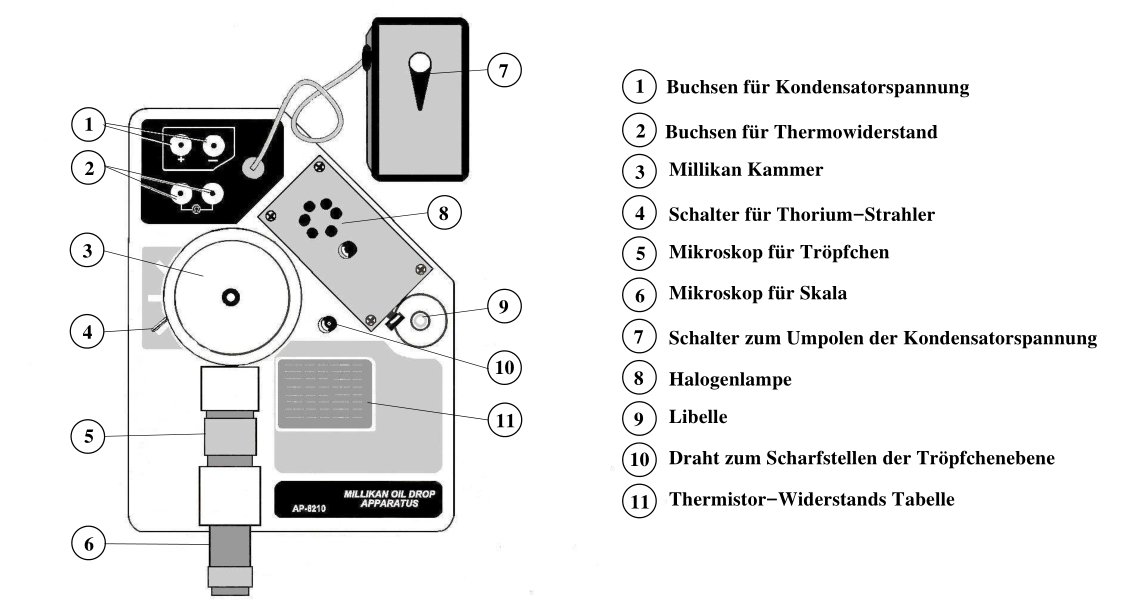
\includegraphics[width=0.5\textwidth]{Abbildungen/Abb_2.png}
    \caption {Schematischer Aufbau des Millikan-Versuchs\cite[3]{V503}.}
    \label{fig:Abb_2}
\end{figure}
Wie in \autoref{sec:Theorie} beschrieben werden die Öltröpfchen teilweise durch das Zerstäuben 
elektrisch geladen. Ist ein messbares Tröpfchen vorhanden, wird die Zeit gemessen, die 
das Tröpfchen benötigt eine zuvor gewählte Strecke zu durchlaufen.
Es wird einmal $t_0$ gemessen, wo das Teilchen ohne Einfluss des elektrischen Feldes fällt.
Anschließend wird für das Tröpfchen drei mal die Steigzeit $t_{auf}$, bei angelegtem positiven Feld und drei mal die Fallzeit $t_{ab}$,
bei angelegtem negativen Feld gemessen. Die Zeiten werden in eine Tabelle eingetragen.\\
Die Messung wird für fünf Tröpfchen bei fünf verschiedenen Spannungen durchgeführt.
\begin{figure}[H]
    \centering
    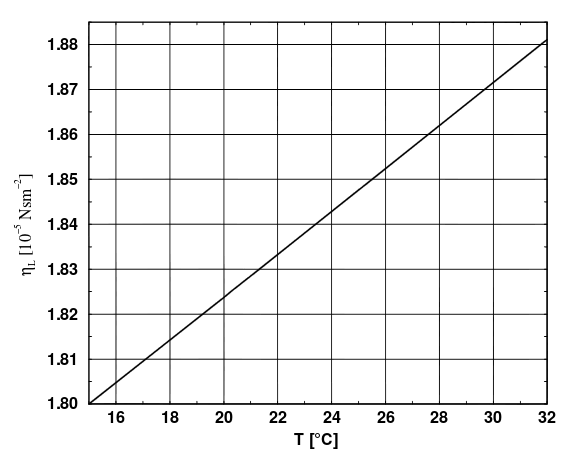
\includegraphics[width=0.5\textwidth]{Abbildungen/Abb_3.png}
    \caption {Viskosität von Luft in Abhängigkeit von der Temperatur\cite[5]{V503}.}
    \label{fig:Abb_3}
\end{figure}